\documentclass[11pt,spanish]{article} % Tipo y tamaño de letra del documento.


\usepackage[utf8]{inputenc}
\usepackage{subfiles}
\usepackage{biblatex}
\addbibresource{references.bib}
\usepackage{multicol}
\usepackage{amsfonts}
\usepackage{blindtext}
\usepackage{mathrsfs}
\usepackage{amsmath}
\usepackage{siunitx}
\usepackage{centernot}
\usepackage[shortlabels]{enumitem}
\usepackage{subfig}
\usepackage{datetime}
\usepackage{listingsutf8}
\usepackage[spanish]{babel}
\usepackage{tikz}
\usepackage{hyperref}
\usepackage[vlined,ruled,linesnumbered]{algorithm2e}
\usepackage{listings}
\usepackage{float}
\usepackage{url}
\usepackage{csquotes}
\usepackage{fourier} %font
\usepackage[top=2cm, bottom=2cm, left=2.5cm, right=2.5cm]{geometry}
\usepackage{pgfplots}
\usepackage{fancyhdr}
\usepackage{mdframed}
\usepackage{tikzducks}
\usepackage[nameinlink]{cleveref}
\usepackage{epigraph} 

\pgfplotsset{compat=1.18}

\usetikzlibrary{shapes.arrows, shapes.geometric, arrows.meta,angles,quotes,positioning,arrows,fit,quotes,calc}
\tikzset{>=latex} 

\setlength\algomargin{1em} 
\SetFuncSty{sc} 
\SetCommentSty{em} 


\Crefname{figure}{Fig.}{Figs.}
\newcommand\crefrangeconjunction{--}
\Crefname{table}{Tabla}{Tablas}
\Crefname{subsubsection}{Subsubsec.}{Subsubsections}
\Crefname{subsection}{Subsec.}{Subsections}
\Crefname{section}{Sec.}{Sections}
\Crefname{equation}{eq.}{eqs.}
\crefname{thm}{Theorem}{theorems}
\Crefname{thm}{Theorem}{Theorems} 

\definecolor{algoco}{rgb}{0,0.4,1}

\hypersetup{
  colorlinks=true,
  linkcolor=algoco,
  citecolor=blue,
  urlcolor=blue,
}

\lstset{
extendedchars=true
inputencoding=utf8/latin1,
basicstyle=\footnotesize\sffamily\color{black},
commentstyle=\slshape \color{gray},
numbers=left,
numbersep=10pt,
numberstyle=\tiny\color{red!80!black},
keywordstyle=\color{red!80!magenta},
showspaces=false,
showstringspaces=false,
stringstyle=\color{cyan!80!black},
tabsize=2,
literate={á}{{\'a}}1 {é}{{\'e}}1 {í}{{\'i}}1 {ó}{{\'o}}1 {ú}{{\'u}}1,
frame = single, 
numbers = none,
float, floatplacement = ht, captionpos = b,
xleftmargin = 2em, xrightmargin = 2em, 
}

\newcommand{\ub}[1]{\underbrace{#1}}
\newcommand\tcm{\textcolor{magenta}}
\newcommand\tca{\textcolor{algoco}}

\setlength\epigraphwidth{.7\textwidth} 

\newcommand{\tnum}{2 y 3} % reemplace 2 por el número de la tarea
\newcommand{\sem}{2024-2} % reemplace 2024-2 por el semestre correspondiente
\newcommand{\campus}{Sede San Joaquin \\ Santiago} % reemplace Casa Central por el campus correspondiente
\newcommand{\rolusm}{202273539-2} % reemplace 2025073100-1 por su rol
\newcommand{\namestudent}{Damian Alexander Rojas Robles} % reemplace Al Goritmo Pérez por su nombre

\headheight=14pt
\linespread{1.3}
\author{\namestudent}
\pagestyle{fancy}
\fancyhf{}%
\fancyfoot[R]{ \namestudent \\ \rolusm}
\fancyfoot[L]{Campus \campus} 
\fancyfoot[C]{\thepage}
\rhead{2024-2}
\lhead{INF-221}
\renewcommand{\headrulewidth}{0.4pt}
\renewcommand{\footrulewidth}{0.4pt}
\newbool{programs}
\boolfalse{programs}
\chead{REPORTE TAREA \tnum~}



\title{
  \huge
  \textbf{REPORTE TAREA \tnum~ \\ ALGORITMOS Y COMPLEJIDAD} \\[1ex]
  \emph{\textquote{Explorando la Distancia entre Cadenas, una Operación a la Vez}}
  }

  
\date{
  \small
  \today\\
  \currenttime
}




\begin{document}
\maketitle
\thispagestyle{fancy} 
\vspace{-1.0\baselineskip}




\begin{abstract}
  \textit{ 
    Este informe presenta dos enfoques para resolver el problema de transformación de cadenas: fuerza bruta y programación dinámica. La implementación en fuerza bruta utiliza recursión para explorar todas las combinaciones posibles de operaciones (sustitución, inserción, eliminación y transposición), pero su complejidad exponencial la hace impráctica para cadenas largas. En contraste, la programación dinámica optimiza el proceso utilizando una matriz para almacenar costos intermedios, logrando una mayor eficiencia.

La evaluación experimental se realizó en un equipo con especificaciones específicas, utilizando pruebas de tiempo y validación de costos. Los resultados muestran que la programación dinámica es considerablemente más rápida y eficiente en términos de memoria, especialmente para cadenas más largas.
  }
     
\end{abstract}

\setcounter{tocdepth}{1}
\tableofcontents


\newpage
\section{Introducción}

El diseño y análisis de algoritmos es una de las áreas más importantes en Ciencias de la Computación. Nos permite comprender cómo funcionan las soluciones a problemas reales y encontrar formas de hacerlas más rápidas y eficientes. Este campo ayuda a mejorar el rendimiento de los programas y que asegura que puedan manejar grandes cantidades de datos o funcionar bien incluso cuando los recursos son limitados. Un ejemplo interesante es el estudio de problemas relacionados con la transformación de cadenas, como calcular el costo más bajo para convertir una cadena en otra usando ciertas operaciones. Este tipo de problemas tiene aplicaciones prácticas en cosas como la edición de texto, lo que lo hace especialmente valioso.
\newline
A lo largo del tiempo, se han creado diferentes formas de abordar estos problemas. Al principio, se usaban métodos sencillos, como los algoritmos de fuerza bruta, que aunque fáciles de implementar, se vuelven poco eficientes cuando las entradas son muy grandes. La programación dinámica ofreció una mejora al almacenar y reutilizar resultados intermedios, lo que hace que los algoritmos sean mucho más rápidos y consuman menos recursos. 
\newline
Este informe tiene como objetivo analizar y comparar dos algoritmos para la transformación de cadenas: el de fuerza bruta y el de programación dinámica. La idea principal es que, aunque la programación dinámica es generalmente más eficiente para cadenas largas, el enfoque de fuerza bruta podría ser más competitivo en casos específicos, como cuando las entradas son pequeñas o las cadenas tienen mucha similitud entre sí. Para poner a prueba esta idea, se implementarán ambos métodos, se medirán sus tiempos de ejecución en diferentes situaciones y se evaluará qué tan precisos son al calcular los costos mínimos de transformación.

\newpage
\section{Diseño y Análisis de Algoritmos} 
%\begin{mdframed}
    \textbf{La extensión máxima para esta sección es de 5 páginas.}
\end{mdframed}

Diseñar un algoritmo por cada técnica de diseño de algoritmos mencionada en la sección de objetivos. Cada algoritmo debe resolver el problema de distancia mínima de edición extendida, dadas dos cadenas \texttt{S1} y \texttt{S2}, utilizando las operaciones y costos especificados.

\begin{itemize}
    \item Describir la solución diseñada. 
    \item Incluir pseudocódigo (ver ejemplo \cref{alg:mi_algoritmo_1})
    \item Proporciones un ejemplo paso a paso de la ejecución de sus algoritmos que ilustren cómo sus algoritmos manejan diferentes escenarios, particularmente donde las
    transposiciones o los costos variables afectan el
    resultado. Haga referencias a los programas expresados en psudocódigo (además puede hacer diagramas).
    \item Analizar la Complejidad temporal y espacial de los algoritmos diseñados en términos de las longitudes de las cadenas de entrada $S1$ y $S2$
    \item Discute cómo la inclusión de transposiciones y costos   variables impacta la complejidad.
\end{itemize}

Los pseudocódigos los he diseñado utilizando el paquete \citetitle{algorithm2e} \cite{algorithm2e} para la presentación de algoritmos. Se recomienda consultar \citetitle{ctan-algorithm2e} \cite{ctan-algorithm2e} y \citetitle{overleaf-algorithms} \cite{overleaf-algorithms}.

Todo lo correspondiente a esta sección es, digamos, en ``\href{https://dle.rae.es/metáfora}{lapiz y papel}'', en el sentido de que no necesita de implementaciones ni resultados experimentales. 

\begin{mdframed}
    Recuerde que lo importante es diseñar algoritmos que cumplan con los paradigmas especificados. 
\end{mdframed}

\begin{mdframed}
    Si se utiliza algún código, idea, o contenido extraído de otra fuente, este \textbf{debe} ser citado en el lugar exacto donde se utilice, en lugar de mencionarlo al final del informe. 
\end{mdframed}


%\newpage
\subsection{Fuerza Bruta}
\epigraph{\textit{``Indeed, brute force is a perfectly good technique in many cases; the real question is, can we use brute force in such a way that we avoid the worst-case behavior?''}}{--- \citeauthor{taocv3}, \citeyear{taocv3} \cite{taocv3}}
Esta solución busca el menor costo para transformar una cadena de caracteres `origen` en otra cadena `objetivo`. Cada operación tiene un costo asignado: la sustitución cuesta 2 si los caracteres son diferentes, la inserción y eliminación cuestan 1, y la transposición cuesta 1. La función `transformar` es recursiva y evalúa todas las posibles transformaciones aplicables en cada posición de las cadenas. Como tal, el programa no transforma el string, sino que calcula directamente el costo de estas operaciones.
\\
El programa ejecuta cada una de las posibilidades para cada caracter del string, ejecutando todas las opciones y eligiendo la menor de estas. En el siguiente ejemplo se revisa un camino optimo en donde vemos el costo de transformar 'plomero' a 'polimeros'

\vspace{1em} % Espacio adicional para separación

\begin{figure}[h]
    \centering
    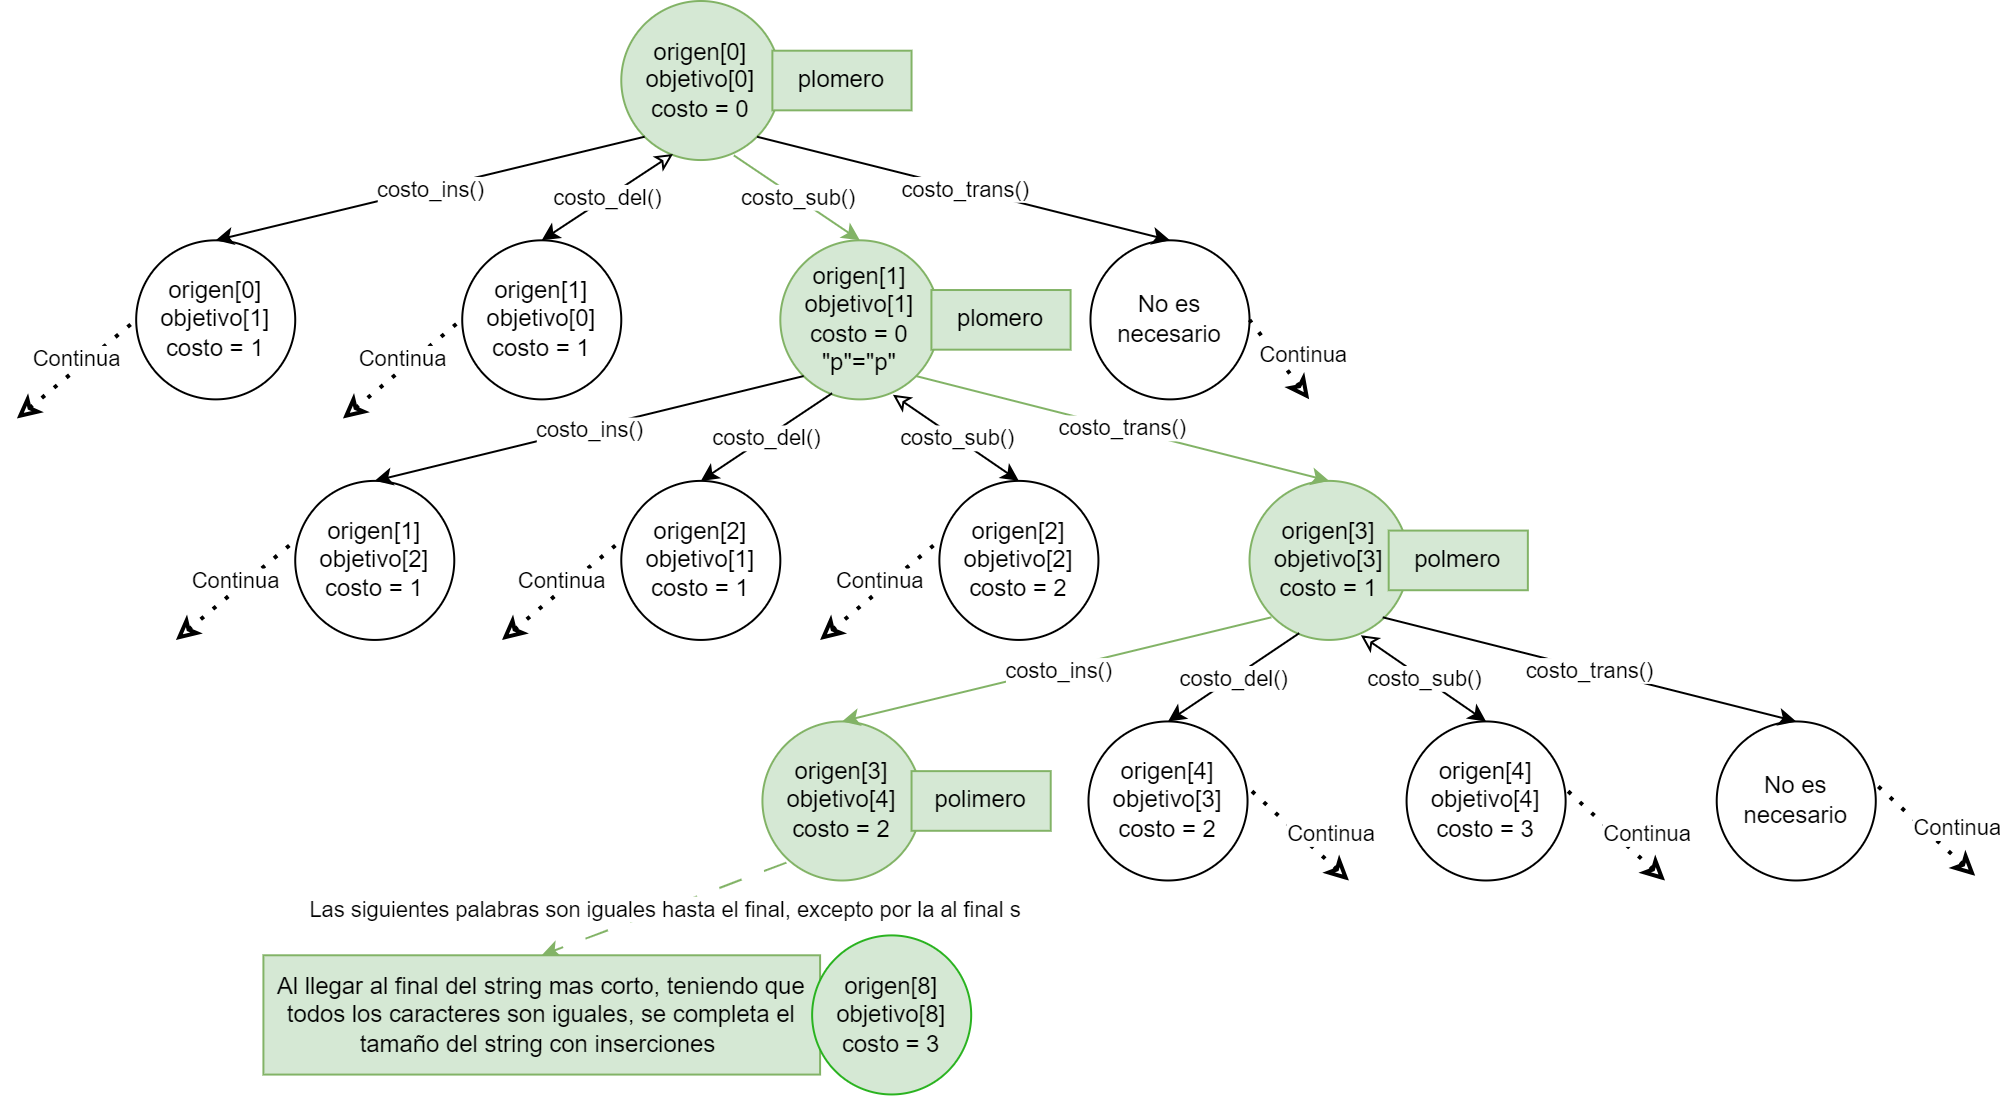
\includegraphics[width=1\linewidth]{AlgoReportTemplate-main/images/Bruteforce Plomero-Polimeros.png}
    \label{fig:enter-label}
\end{figure}
El programa revisa todos los casos posible en el string recursivamente, llegando al ultimo caracter del string, donde retorna en caso de que haya una diferencia en el tamaño del string. cuando llega al nivel mas abajo, comienza a evaluar, retornando el costo de cada transformacion.
\\
\begin{algorithm}[H]
    \SetKwProg{myproc}{Procedure}{}{}
    \SetKwFunction{AlgorithmName}{Transformar}  % Cambia 'AlgorithmName' por el nombre del enfoque elegido
    \SetKwFunction{CostoSub}{costo\_sub}  % Función auxiliar de ejemplo
    \SetKwFunction{CostoIns}{costo\_ins}
    \SetKwFunction{CostoDel}{costo\_del}
    \SetKwFunction{CostoTrans}{costo\_trans}
    \DontPrintSemicolon
    \footnotesize

    % Definición del algoritmo principal
    \myproc{\AlgorithmName{origen, objetivo, i, j, costo\_acumulado}}{
    \uIf{$i =$ longitud de origen y $j =$ longitud de objetivo}{
        \Return costo\_acumulado\;  % Fin de la transformación
    }
    \uElseIf{$i =$ longitud de origen}{
        \Return costo\_acumulado + (longitud de objetivo - $j$)\;  % Coste por inserciones restantes
    }
    \uElseIf{$j =$ longitud de objetivo}{
        \Return costo\_acumulado + (longitud de origen - $i$)\;  % Coste por eliminaciones restantes
    }

    % Caso base: cálculo de costo mínimo
    $costo\_min \leftarrow \infty$\;

    % Costo de sustitución
    $costo\_sust \leftarrow costo\_acumulado + \CostoSub{origen[i], objetivo[j]}$\;
    $costo\_min \leftarrow \min(costo\_min, \AlgorithmName{origen, objetivo, i+1, j+1, costo\_sust})$\;

    % Costo de inserción
    $costo\_inser \leftarrow costo\_acumulado + \CostoIns{objetivo[j]}$\;
    $costo\_min \leftarrow \min(costo\_min, \AlgorithmName{origen, objetivo, i, j+1, costo\_inser})$\;

    % Costo de eliminación
    $costo\_elim \leftarrow costo\_acumulado + \CostoDel{origen[i]}$\;
    $costo\_min \leftarrow \min(costo\_min, \AlgorithmName{origen, objetivo, i+1, j, costo\_elim})$\;

    % Costo de transposición
    \uIf{$i+1 <$ longitud de origen y $j+1 <$ longitud de objetivo y origen[i] = objetivo[j+1] y origen[i+1] = objetivo[j]}{
        $costo\_transp \leftarrow costo\_acumulado + \CostoTrans{origen[i], origen[i+1]}$\;
        $costo\_min \leftarrow \min(costo\_min, \AlgorithmName{origen, objetivo, i+2, j+2, costo\_transp})$\;
    }

    \Return costo\_min\;
}

    % Definición de la función auxiliar
    \myproc{\CostoSub{a, b}}{
    \Return \uIf{$a = b$}{0\;} \Else{2\;}
    }
    
    \myproc{\CostoIns{b}}{
        \Return 1\;
    }
    
    \myproc{\CostoDel{a}}{
        \Return 1\;
    }
    
    \myproc{\CostoTrans{a, b}}{
        \Return \uIf{$a = b$}{0\;} \Else{1\;}
    }
    \caption{Algoritmo de transformación por fuerza bruta entre dos cadenas para encontrar el costo mínimo de conversión. (i y j indices de origen y objetivo, respectivamente)}
    \label{alg:mi_algoritmo_1}

\end{algorithm}
El programa tiene un orden temporal de \(O(4^{\min(m, n)})\), ya que por cada carácter realiza 4 llamadas recursivas, repitiendo el mismo proceso. Al llegar al final del string más corto, devuelve la distancia de diferencia con el otro string. Espacialmente, al pasar los strings por referencia, el orden espacial es \(O(m+n)\).

El programa utiliza recursión en los métodos que alteran el string. La sustitución implica eliminar e insertar un elemento, lo cual tiene un costo acorde. Sin embargo, la transposición introduce una recursión adicional, ya que, aunque pueda implicar una eliminación e inserción en posiciones cercanas, su costo justifica evaluarla.
\newpage
\subsection{Programación Dinámica}

\epigraph{\textit{Dynamic programming is not about filling in tables. It's about smart recursion!}}{\citeauthor{algorithms_erickson}, \citeyear{algorithms_erickson} \cite{algorithms_erickson}}

%%%%%%%%%%%%%%%%%%%%%%%%%%%%%%%%%%%%%%%%%%%%%%%%%%%%%%%%%%%%%%
\subsubsection{Descripción de la solución recursiva}
Las funciones de coste funcionan de la misma manera que en el caso anterior, pero con la variación de que la función \texttt{transformar} utiliza programación dinámica para evaluar todas las posibles transformaciones en cada posición de las cadenas, almacenando los costos acumulados de cada subproblema en una matriz para evitar recalcular los mismos valores.

\subsubsection{Relación de recurrencia}
Este código utiliza programación dinámica para calcular el costo mínimo de transformar una cadena \texttt{s1} en otra \texttt{s2}. Para ello, utiliza una matriz \texttt{dp} donde \texttt{dp[i][j]} representa el costo mínimo para transformar los primeros \(i\) caracteres de \texttt{s1} en los primeros \(j\) caracteres de \texttt{s2}. Se definen costos para cuatro operaciones: sustitución, inserción, eliminación y transposición. La matriz se llena iterativamente, evaluando el costo mínimo entre estas operaciones. Al final, \texttt{dp[m][n]} contiene el costo mínimo de la transformación, que se imprime.

\subsubsection{Identificación de subproblemas}
El algoritmo identifica los subproblemas a resolver mediante la partición de las cadenas en segmentos más pequeños. Cada celda de la matriz \texttt{dp} corresponde a un subproblema que calcula el costo de transformar un prefijo de la cadena \texttt{s1} en un prefijo de la cadena \texttt{s2}. Estos subproblemas se resuelven de manera acumulativa, asegurando que los valores previamente calculados sean reutilizados en lugar de recalcularse.

\subsubsection{Estructura de datos y orden de cálculo}
El programa utiliza una matriz bidimensional \texttt{dp} de tamaño \( (m+1) \times (n+1) \), donde \(m\) y \(n\) son las longitudes de las cadenas \texttt{s1} y \texttt{s2}, respectivamente. El cálculo se realiza llenando esta matriz celda por celda, de izquierda a derecha y de arriba hacia abajo. Cada celda \texttt{dp[i][j]} se calcula considerando los costos de las operaciones posibles (sustitución, inserción, eliminación y transposición).

\subsubsection{Algoritmo utilizando programación dinámica}

\begin{itemize}
    \item Inicializa la matriz \texttt{dp} con dimensiones \( (m+1) \times (n+1) \).
    \item Llena la primera fila y la primera columna con valores base, correspondientes a los costos acumulados para transformar cadenas vacías.
    \item Itera sobre los índices \(i\) y \(j\) para calcular el costo mínimo en cada celda \texttt{dp[i][j]}, evaluando las operaciones de transformación.
    \item Al finalizar, el valor en \texttt{dp[m][n]} representa el costo mínimo de transformar \texttt{s1} en \texttt{s2}.
\end{itemize}

\begin{figure}[h]
    \centering
    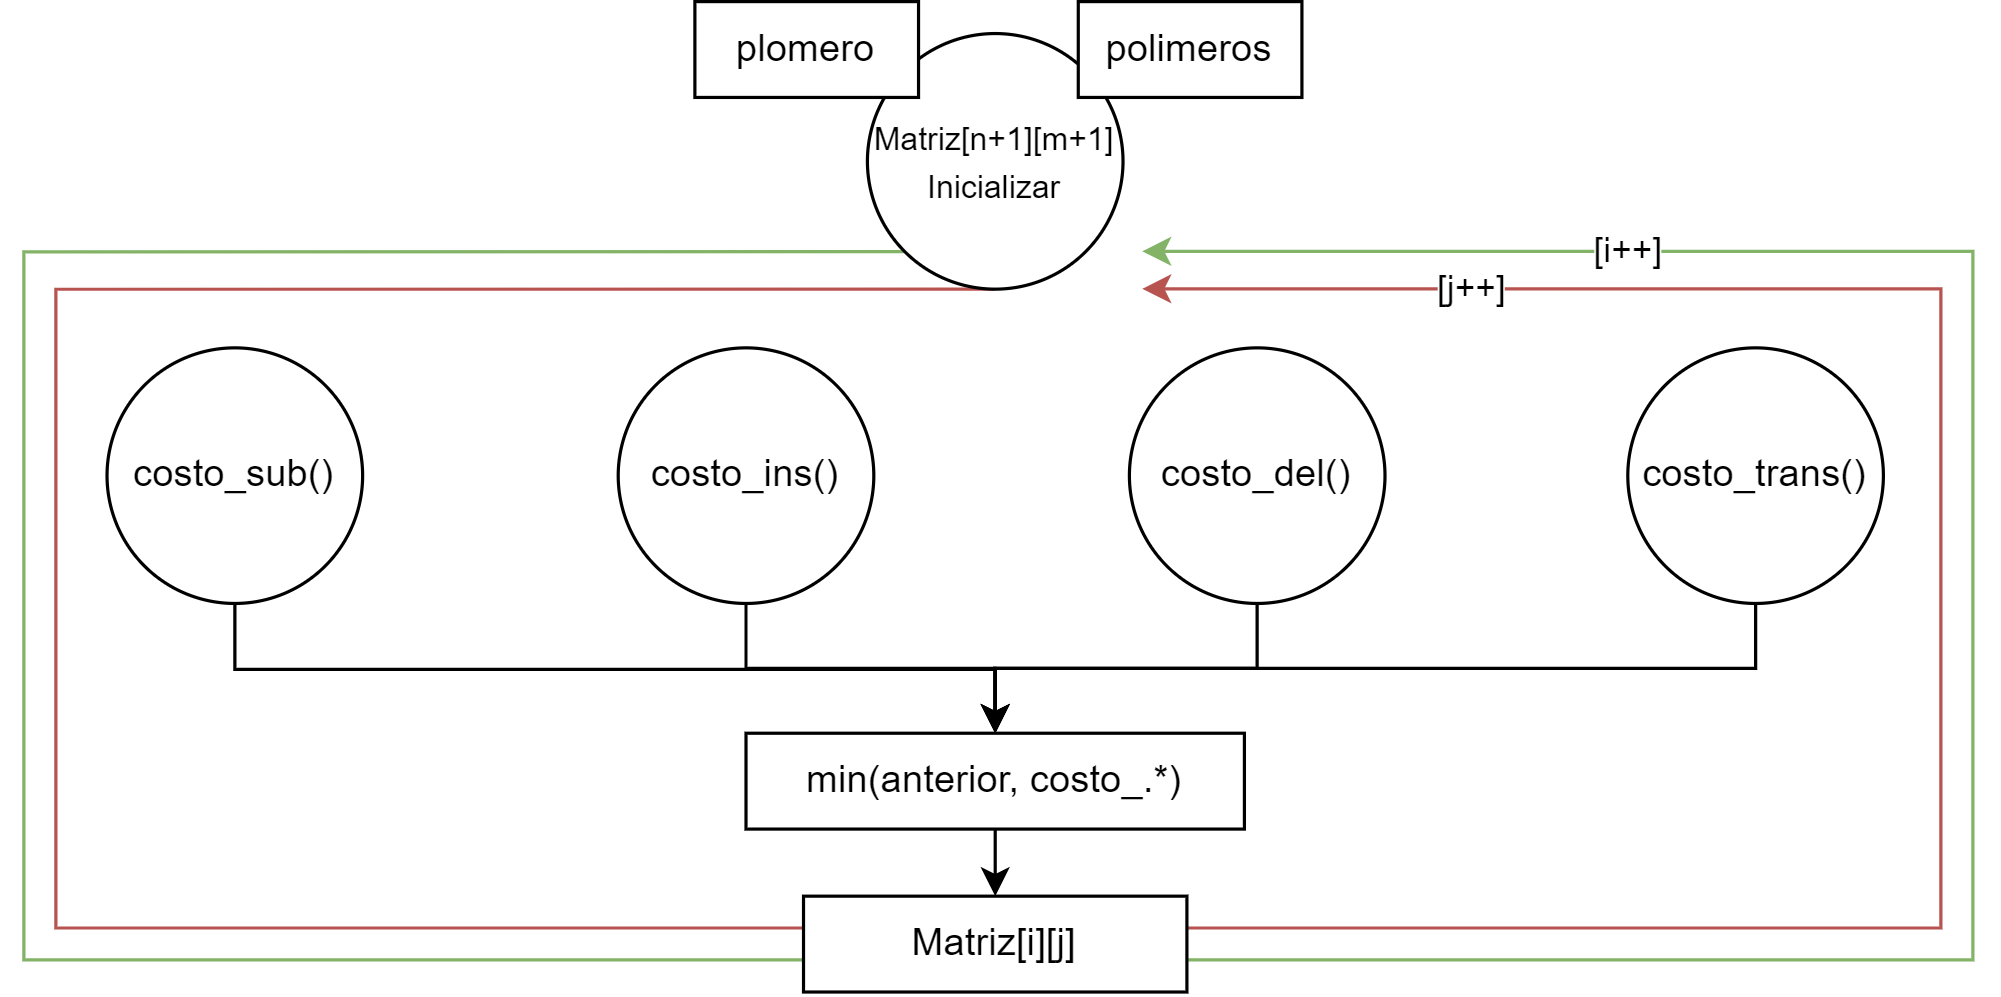
\includegraphics[width=.7\linewidth]{AlgoReportTemplate-main/images/DinamicProgramation.png}
    \caption{Visualización del proceso de programación dinámica.}
\end{figure}

\begin{figure}[h!]
    \centering
    \begin{minipage}{0.45\textwidth}
        \centering
        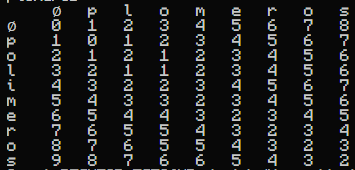
\includegraphics[width=1\linewidth]{AlgoReportTemplate-main/images/Matrix.png}
        \caption{Matriz resultante después de las iteraciones.}
    \end{minipage}%
    \hspace{1em}
    \begin{minipage}{0.45\textwidth}
        Después de completar las iteraciones necesarias, la matriz completa quedaría tal que así. Los valores corresponden al mínimo de la función de transformación, donde \texttt{dp[m][n]} es el valor óptimo.
    \end{minipage}
\end{figure}

\begin{algorithm}[H]
\SetKwProg{myproc}{Procedure}{}{}
    \SetKwFunction{Transformar}{Transformar}  % Cambia 'AlgorithmName' por el nombre del enfoque elegido
    \SetKwFunction{CostoSub}{costo\_sub}  % Función auxiliar de ejemplo
    \SetKwFunction{CostoIns}{costo\_ins}
    \SetKwFunction{CostoDel}{costo\_del}
    \SetKwFunction{CostoTrans}{costo\_trans}
    \DontPrintSemicolon
    \footnotesize

    % Definición del algoritmo principal
    \myproc{\Transformar{s1, s2}}{
    $m \leftarrow$ longitud de s1\;
    $n \leftarrow$ longitud de s2\;

    % Inicializar matriz dp con valores máximos
    Crear matriz $dp$ de tamaño $(m+1) \times (n+1)$ con todos los valores igual a $\infty$\;

    % Configurar condiciones iniciales
    $dp[0][0] \leftarrow 0$\;
    \For{$i \leftarrow 1$ \KwTo $m$}{
        $dp[i][0] \leftarrow dp[i-1][0] + \CostoDel{s1[i-1]}$\;  % Costo de eliminar caracteres de s1
    }
    \For{$j \leftarrow 1$ \KwTo $n$}{
        $dp[0][j] \leftarrow dp[0][j-1] + \CostoIns{s2[j-1]}$\;  % Costo de insertar caracteres de s2
    }

    % Llenar la matriz dp
    \For{$i \leftarrow 1$ \KwTo $m$}{
        \For{$j \leftarrow 1$ \KwTo $n$}{
            % Cálculo de sustitución
            $costo\_sust \leftarrow dp[i-1][j-1] + \CostoSub{s1[i-1], s2[j-1]}$\;
            $dp[i][j] \leftarrow \min(dp[i][j], costo\_sust)$\;

            % Cálculo de inserción
            $costo\_inser \leftarrow dp[i][j-1] + \CostoIns{s2[j-1]}$\;
            $dp[i][j] \leftarrow \min(dp[i][j], costo\_inser)$\;

            % Cálculo de eliminación
            $costo\_elim \leftarrow dp[i-1][j] + \CostoDel{s1[i-1]}$\;
            $dp[i][j] \leftarrow \min(dp[i][j], costo\_elim)$\;

            % Cálculo de transposición
            \uIf{$i > 1$ y $j > 1$ y $s1[i-1] = s2[j-2]$ y $s1[i-2] = s2[j-1]$}{
                $costo\_transp \leftarrow dp[i-2][j-2] + \CostoTrans{s1[i-2], s1[i-1]}$\;
                $dp[i][j] \leftarrow \min(dp[i][j], costo\_transp)$\;
            }
        }
    }

    \Return $dp[m][n]$\;  % Resultado final de la transformación mínima
}


    % Definición de la función auxiliar
    \myproc{\CostoSub{a, b}}{
    \Return \uIf{$a = b$}{0\;} \Else{2\;}
    }
    
    \myproc{\CostoIns{b}}{
        \Return 1\;
    }
    
    \myproc{\CostoDel{a}}{
        \Return 1\;
    }
    
    \myproc{\CostoTrans{a, b}}{
        \Return \uIf{$a = b$}{0\;} \Else{1\;}
    }
    \caption{Algoritmo basado en programación dinámica para calcular el costo mínimo de transformar una cadena \(s1\) en otra cadena \(s2\) mediante tabulacion.}
    \label{alg:mi_algoritmo_2}
\end{algorithm}

El programa tiene un orden temporal de \(O(m \times n)\), donde \(m\) y \(n\) son las longitudes de las cadenas. Esto se debe a que se llena una matriz de tamaño \( (m+1) \times (n+1) \), realizando un número constante de operaciones por celda para calcular los costos de las transformaciones posibles.

El algoritmo tiene un orden espacial de \(O(m \times n)\), ya que utiliza una matriz de tamaño \( (m+1) \times (n+1) \) para almacenar los resultados intermedios.


\newpage
\section{Implementaciones}
La implementación presentada resuelve el problema de transformación de cadenas utilizando dos enfoques distintos: fuerza bruta y programación dinámica. Además, se incluye un script en Bash para automatizar la ejecución de los casos de prueba almacenados en una estructura de carpetas.\\

El archivo `BruteForce.cpp` implementa un enfoque de fuerza bruta mediante recursión, explorando todas las combinaciones posibles de operaciones (sustitución, inserción, eliminación y transposición) para transformar una cadena en otra. Determina el costo mínimo al evaluar cada opción y selecciona la que genera el menor costo acumulado.\\

El archivo `Dinamic.cpp` implementa un enfoque basado en programación dinámica, que es considerablemente más eficiente que la fuerza bruta. Este método utiliza una matriz para almacenar los costos intermedios de transformar subcadenas, eliminando cálculos redundantes. La matriz se llena iterativamente, evaluando todas las operaciones posibles y seleccionando la que minimiza el costo acumulado. Este enfoque tiene una complejidad temporal \(O(m \times n)\), donde \(m\) y \(n\) son las longitudes de las cadenas.\\

El enfoque de fuerza bruta, aunque sencillo, tiene una complejidad exponencial y un uso constante de memoria, lo que lo hace impráctico para cadenas largas. En cambio, la programación dinámica es significativamente más eficiente, con complejidad temporal \(O(m \times n)\) y uso de memoria proporcional al tamaño de las cadenas, siendo más adecuada para aplicaciones reales. No obstante, su implementación es más compleja debido a la necesidad de gestionar y llenar una matriz.\\

El script `test.sh` automatiza la ejecución masiva de pruebas iterando sobre subcarpetas del directorio `testcases/`, donde cada archivo `test.txt` contiene dos cadenas de prueba. Ejecuta el programa `main` con estos datos como entrada estándar y muestra los resultados, permitiendo comparar resultados o medir tiempos eficientemente.

\newpage
\section{Experimentos}

\epigraph{``\textit{Non-reproducible single occurrences are of no significance to
science.}''}{---\citeauthor{popper2005logic},\citeyear{popper2005logic} \cite{popper2005logic}}

Para la experimentación y evaluación del desempeño del algoritmo propuesto, se utilizó un equipo con las siguientes especificaciones técnicas:

\begin{itemize}
    \item \textbf{Sistema Operativo:} Windows 10 Home Single Language, 64 bits (versión 10.0, compilación 19045).
    \item \textbf{Procesador:} Intel® Core™ i5-10300H CPU @ 2.50GHz (8 núcleos).
    \item \textbf{Memoria RAM:} 16 GB (16384 MB).
    \item \textbf{Disco Duro:} Unidad NVMe SSD de 512 GB.
    \item \textbf{Tarjeta Gráfica:} NVIDIA GeForce GTX 1650. 
\end{itemize}

 

El programa utiliza las librerias estandar de c++, el uso de la libreria <string>, para manejo de los string de entrada. Especificamente en el programa de fuerza bruta, se utiliza la libreria <limits>, ya que se utiliza para conseguir el valor maximo perimitido por un int. En la solucion por programacion dinamica se utiliza la lirberia <vector> para lacreacion y manejo de la matriz para la resolucion del problema. Ademas de que se uso la libreria <chrono> para el calculo temporal de las funciones a la hora de resolver los distintos casos. Se utilizó un entorno WSL para la ejecucion de los programas.

\subsection{Dataset (casos de prueba)}
\subsection*{Pruebas realizadas}

Para la experimentación actual, implementamos dos tipos principales de pruebas:

\begin{enumerate}
    \item \textbf{Prueba temporal:}  
    En esta prueba, nos enfocamos en medir el tiempo que cada método (fuerza bruta y programación dinámica) tarda en resolver una serie de ejercicios generados mediante programas en Python, independientemente del resultado de la función. Los casos evaluados incluyen:  
    \begin{itemize}
        \item \textbf{Cadenas de distintos tamaños}
        \item \textbf{Cadenas completamente iguales}
        \item \textbf{Una cadena vacía y otra no vacía}  
        \item \textbf{Cadenas de igual tamaño pero con letras completamente distintas}  
        \item \textbf{Entradas que solo pueden resolverse mediante transposición}  
    \end{itemize}
    Este enfoque permitió comparar directamente los tiempos de ejecución entre ambos métodos en diferentes escenarios.

    \item \textbf{Prueba de validación de costos:}  
    En esta prueba utilizamos un dataset limitado con entradas seleccionadas y cuales resultados esperados fueron calculados manualmente. Posteriormente, comparamos estos valores con los resultados obtenidos por el programa, asegurándonos de que los costos fueran correctos en todos los casos.
\end{enumerate}

Estas pruebas nos permitieron analizar la eficiencia en términos de rendimiento.

\subsubsection*{Ejemplos de entradas para pruebas}

A continuación, se presentan ejemplos de entradas utilizadas para evaluar el rendimiento y la precisión del algoritmo, clasificados según las características de las cadenas:

\begin{enumerate}
    \item \textbf{Cadenas de distintos tamaños:}
    \begin{itemize}
        \item Entrada:
        \begin{verbatim}
        "st"
        "abcdef"
        \end{verbatim}
        \item Explicación: Una cadena es significativamente más grande que la otra, lo que genera múltiples inserciones.
    \end{itemize}

    \item \textbf{Cadenas completamente iguales:}
    \begin{itemize}
        \item Entrada:
        \begin{verbatim}
        "algoritmo"
        "algoritmo"
        \end{verbatim}
        \item Explicación: Ambas cadenas son idénticas, lo que debería resultar en un costo de transformación igual a cero.
    \end{itemize}

    \item \textbf{Una cadena vacía y otra no vacía:}
    \begin{itemize}
        \item Entrada:
        \begin{verbatim}
        ""
        "transformar"
        \end{verbatim}
        \item Explicación: Una de las cadenas está vacía, lo que implica que todas las operaciones serán inserciones.
    \end{itemize}

    \item \textbf{Cadenas de igual tamaño pero con letras completamente distintas:}
    \begin{itemize}
        \item Entrada:
        \begin{verbatim}
        "abcde"
        "vwxyz"
        \end{verbatim}
        \item Explicación: Ambas cadenas tienen el mismo tamaño, pero no tienen caracteres en común, por lo que el resultado implicará únicamente sustituciones.
    \end{itemize}

    \item \textbf{Entradas que solo pueden resolverse mediante transposición:}
    \begin{itemize}
        \item Entrada:
        \begin{verbatim}
        "ab"
        "ba"
        \end{verbatim}
        \item Explicación: Las cadenas son iguales en contenido pero tienen los caracteres intercambiados, lo que hace necesario el uso de la operación de transposición.
    \end{itemize}
\end{enumerate}


\newpage
\subsection{Resultados}
En esta sección se presentan los resultados experimentales obtenidos para evaluar el rendimiento de los algoritmos presentados. Los resultados se resumen en las tablas a continuacion, armadas con los tiempos promedio en milisegundos [\textit{ms}] para cada categoría y diferentes tamaños de entrada. Para cada tamaño, se realizaron tres pruebas independientes (\textit{test1}, \textit{test2}, y \textit{test3}) cuyos valores se promediaron para destacar el comportamiento general del algoritmo. Los tiempos destacados en \textbf{negrita} representan los valores promedio obtenidos.

\subsubsection*{Fuerza Bruta}
La tabla muestra los resultados obtenidos al probar el algoritmo de fuerza bruta con diferentes tipos de casos. Este método, aunque simple en su concepto, examina todas las posibles formas de transformar una cadena en otra y elige la que tiene el menor costo. Sin embargo, debido a que utiliza recursión y tiene una complejidad exponencial, el tiempo que tarda en ejecutarse puede variar mucho dependiendo de la longitud y las características de las cadenas analizadas.

\begin{table}[h]
\centering
\scalebox{0.9}{
\begin{tabular}{c|ccccc}
& \textbf{Distinto Tam. [ms]} & \textbf{Str Iguales [ms]} & \textbf{1 Str Vacío [ms]} & \textbf{Distintos Str [ms]} & \textbf{Solo Transposición [ms]} \\ \hline
\textbf{5} & \textbf{0.209766667} & \textbf{0.2022} & \textbf{0.001} & \textbf{0.2143} & \textbf{0.206066667} \\ \hline
test1 & 0.1994 & 0.1985 & 0.001 & 0.2086 & 0.1988 \\
test2 & 0.2307 & 0.2036 & 0.0011 & 0.2351 & 0.1992 \\
test3 & 0.1992 & 0.2045 & 0.001 & 0.1992 & 0.1995 \\ \hline
\textbf{6} & \textbf{0.214666667} & \textbf{1.151733333} & \textbf{0.00166667} & \textbf{1.084166667} & \textbf{1.0974} \\ \hline
test1 & 0.2421 & 1.1352 & 0.001 & 1.0851 & 1.0847 \\
test2 & 0.1992 & 1.1225 & 0.0009 & 1.0812 & 1.1227 \\
test3 & 0.2081 & 1.1251 & 0.001 & 1.0814 & 1.1258 \\ \hline
\textbf{7} & \textbf{4.302233333} & \textbf{6.211533333} & \textbf{0.000966667} & \textbf{6.0378} & \textbf{6.062966667} \\ \hline
test1 & 6.9041 & 6.5234 & 0.001 & 6.448 & 6.4338 \\
test2 & 6.1986 & 6.077 & 0.001 & 6.4517 & 6.0974 \\
test3 & 5.9828 & 6.0432 & 0.001 & 6.4493 & 6.0722 \\ \hline
\textbf{8} & \textbf{14.01323333} & \textbf{34.0214} & \textbf{0.00133333} & \textbf{33.5678} & \textbf{35.26496667} \\ \hline
test1 & 5.0211 & 34.3423 & 0.0011 & 32.8275 & 33.8369 \\
test2 & 1.6996 & 33.1743 & 0.001 & 32.9435 & 34.9697 \\
test3 & 35.319 & 34.5429 & 0.0011 & 33.9435 & 34.9375 \\ \hline
\textbf{9} & \textbf{51.67986667} & \textbf{198.698} & \textbf{0.00113333} & \textbf{184.9345667} & \textbf{192.8536667} \\ \hline
test1 & 77.7683 & 222.328 & 0.001 & 185.553 & 190.984 \\
test2 & 74.2817 & 189.866 & 0.0011 & 185.829 & 182.521 \\
test3 & 2.9984 & 183.9 & 0.001 & 183.422 & 205.002 \\

\end{tabular}
}
\end{table}

\begin{figure}[H]
    \centering
    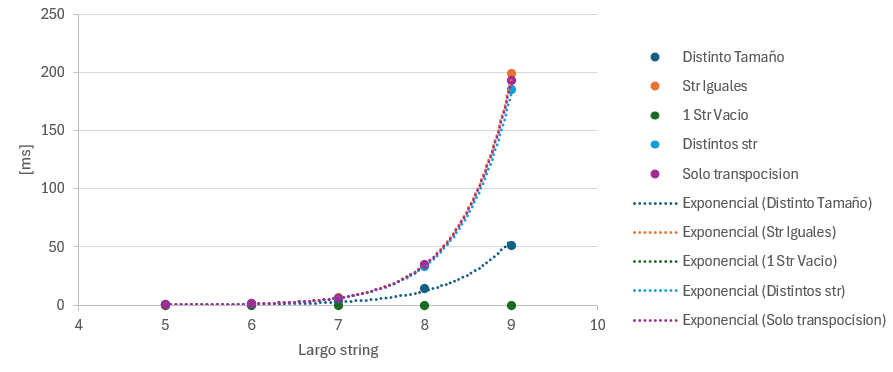
\includegraphics[width=1\linewidth]{AlgoReportTemplate-main//images/GraphBruteForce.png}
    \label{fig:enter-label}
\end{figure}
\vspace{5px}

\subsubsection*{Casos de prueba base}
Se utilizaron varios casos de prueba básicos para evaluar el rendimiento del código de programación dinámica. Estos casos consisten en diferentes configuraciones de entrada, donde se varían características clave del algoritmo. Los resultados de las pruebas se presentan en la siguiente tabla.
\begin{table}[h]
\centering
\scalebox{0.9}{
\begin{tabular}{c|l|c}

\textbf{Prueba} & \textbf{Cadenas} & \textbf{Resultado} \\ \hline
\textbf{1} & 
\begin{tabular}[c]{@{}l@{}}
\texttt{ } \\ 
\texttt{ } \\ 
\end{tabular} & \textbf{0} \\ \hline

\textbf{2} & 
\begin{tabular}[c]{@{}l@{}}
\texttt{nada} \\ 
\texttt{anda} \\ 
\end{tabular} & \textbf{1} \\ \hline

\textbf{3} & 
\begin{tabular}[c]{@{}l@{}}
\texttt{componentes} \\ 
\texttt{comerciales} \\ 
\end{tabular} & \textbf{10} \\ \hline

\textbf{4} & 
\begin{tabular}[c]{@{}l@{}}
\texttt{datos} \\ 
\texttt{estructuras} \\ 
\end{tabular} & \textbf{12} \\ \hline

\textbf{5} & 
\begin{tabular}[c]{@{}l@{}}
\texttt{hola} \\ 
\texttt{ } \\ 
\end{tabular} & \textbf{4} \\

\end{tabular}
}
\end{table}

\subsubsection*{Programacion Dinamica}

La tabla presenta los resultados experimentales obtenidos al aplicar el algoritmo basado en Programación Dinámica a distintos casos de prueba. Este enfoque optimiza el proceso de transformación al almacenar y reutilizar soluciones a subproblemas, lo que reduce significativamente la cantidad de cálculos redundantes en comparación con métodos más simples como el de fuerza bruta. Gracias a esta técnica, el algoritmo logra una complejidad polinómica, haciendo que su tiempo de ejecución sea mucho más eficiente, incluso para cadenas de mayor longitud o complejidad.

\begin{table}[h]
\centering
\scalebox{0.9}{
\begin{tabular}{c|ccccc}

& \textbf{Distinto Tam.} & \textbf{Str Iguales} & \textbf{1 Str Vacío} & \textbf{Distintos Str} & \textbf{Solo Transposición} \\ \hline
\textbf{5} & \textbf{0.0132} & \textbf{0.013033333} & \textbf{0.009566667} & \textbf{0.011733333} & \textbf{0.0104} \\ \hline
test1 & 0.0145 & 0.0132 & 0.0108 & 0.0144 & 0.0111 \\
test2 & 0.0101 & 0.0113 & 0.005 & 0.0104 & 0.0111 \\
test3 & 0.0131 & 0.0121 & 0.0114 & 0.0105 & 0.011 \\ \hline
\textbf{6} & \textbf{0.011733333} & \textbf{0.012066667} & \textbf{0.008933333} & \textbf{0.0131} & \textbf{0.012466667} \\ \hline
test1 & 0.0121 & 0.0122 & 0.0101 & 0.0141 & 0.0114 \\
test2 & 0.0102 & 0.0115 & 0.008 & 0.011 & 0.0115 \\
test3 & 0.0131 & 0.0124 & 0.0099 & 0.0119 & 0.013 \\ \hline
\textbf{7} & \textbf{0.024733333} & \textbf{0.012066667} & \textbf{0.009133333} & \textbf{0.013133333} & \textbf{0.013766667} \\ \hline
test1 & 0.0319 & 0.0131 & 0.011 & 0.0152 & 0.0143 \\
test2 & 0.0112 & 0.0122 & 0.008 & 0.012 & 0.0115 \\
test3 & 0.0106 & 0.0116 & 0.009 & 0.015 & 0.0132 \\ \hline
\textbf{8} & \textbf{0.014833333} & \textbf{0.014333333} & \textbf{0.010333333} & \textbf{0.013066667} & \textbf{0.015033333} \\ \hline
test1 & 0.0112 & 0.0146 & 0.0101 & 0.0128 & 0.0143 \\
test2 & 0.0123 & 0.014 & 0.0099 & 0.0125 & 0.0139 \\
test3 & 0.0131 & 0.0143 & 0.0098 & 0.013 & 0.0147 \\ \hline
\textbf{9} & \textbf{0.0132} & \textbf{0.0146} & \textbf{0.0114} & \textbf{0.015} & \textbf{0.020866667} \\ \hline
test1 & 0.013 & 0.0143 & 0.0108 & 0.0149 & 0.0238 \\
test2 & 0.0129 & 0.0139 & 0.011 & 0.0126 & 0.0166 \\
test3 & 0.0111 & 0.0168 & 0.0107 & 0.0162 & 0.0222 \\

\end{tabular}
}
\end{table}

\begin{figure}[H]
    \centering
    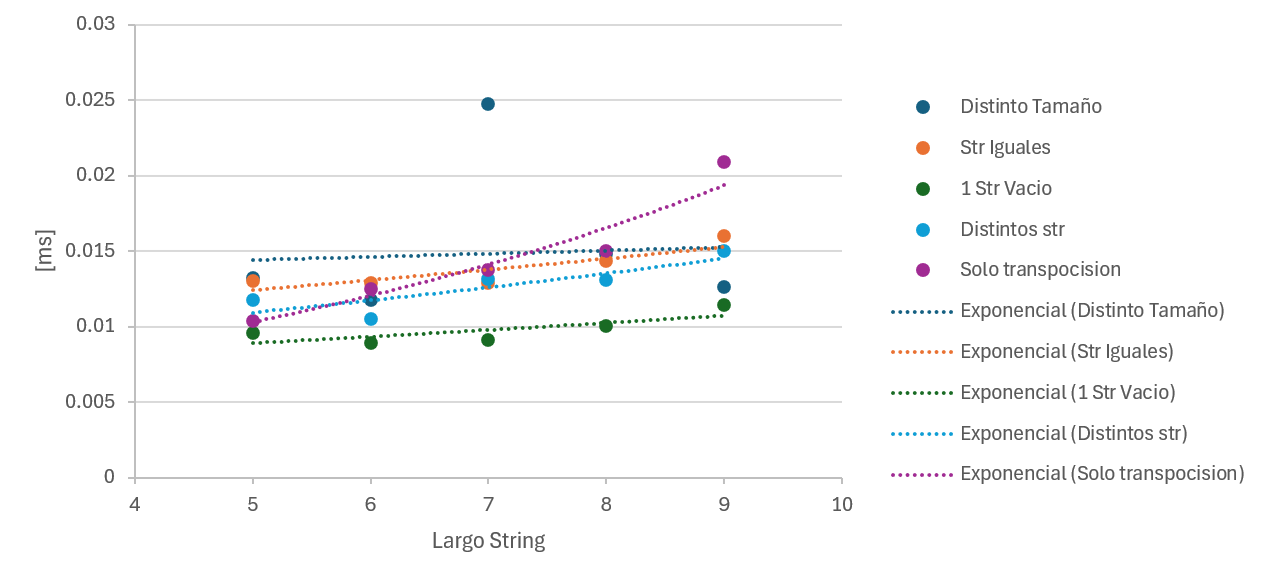
\includegraphics[width=1\linewidth]{AlgoReportTemplate-main//images/graphDP.png}
    \label{fig:enter-label}
\end{figure}

\subsubsection*{Casos de prueba base}

Al igual que en el caso de la fuerza bruta, se evaluo el codigo frente a casos de prueba bases, en los que se variaban caracteristicas importantes del codigo.
Los resultaos se prensentan en la siguiente tabla.

\begin{table}[h]
\centering
\scalebox{0.9}{
\begin{tabular}{c|l|c}

\textbf{Prueba} & \textbf{Cadenas} & \textbf{Resultado} \\ \hline
\textbf{1} & 
\begin{tabular}[c]{@{}l@{}}
\texttt{ } \\ 
\texttt{ } \\ 
\end{tabular} & \textbf{0} \\ \hline

\textbf{2} & 
\begin{tabular}[c]{@{}l@{}}
\texttt{nada} \\ 
\texttt{anda} \\ 
\end{tabular} & \textbf{1} \\ \hline

\textbf{3} & 
\begin{tabular}[c]{@{}l@{}}
\texttt{componentes} \\ 
\texttt{comerciales} \\ 
\end{tabular} & \textbf{10} \\ \hline

\textbf{4} & 
\begin{tabular}[c]{@{}l@{}}
\texttt{datos} \\ 
\texttt{estructuras} \\ 
\end{tabular} & \textbf{12} \\ \hline

\textbf{5} & 
\begin{tabular}[c]{@{}l@{}}
\texttt{hola} \\ 
\texttt{ } \\ 
\end{tabular} & \textbf{4} \\

\end{tabular}
}
\end{table}

\newpage
\section{Conclusiones}


En conclusión, los resultados muestran claramente las diferencias en el rendimiento entre los enfoques de fuerza bruta y programación dinámica para la transformación de cadenas. La solución de fuerza bruta, aunque efectiva en pequeños conjuntos de datos, tiene una complejidad exponencial que la hace ineficiente para cadenas más largas. Por otro lado, la programación dinámica ofrece una solución mucho más eficiente, con una complejidad temporal de O(m × n), lo que la hace ideal para aplicaciones prácticas. Este análisis resalta la importancia de elegir el enfoque adecuado según el tamaño y las características de los datos, lo que mejora considerablemente el rendimiento en situaciones reales. Las pruebas experimentales confirmaron que la programación dinámica no solo reduce el tiempo de ejecución, sino que también optimiza el uso de memoria, lo que la hace más adecuada para trabajar con grandes volúmenes de datos. Aunque ambos métodos tienen su utilidad, la programación dinámica destaca como la opción preferida cuando se busca eficiencia y escalabilidad.

\newpage

\section{Condiciones de entrega}
% Condiciones generales de tareas de Algoritmos y Complejidad, 20231
  \begin{itemize}
  \item
    La tarea se realizará \tca{individualmente}
    (esto es grupos de una persona),
    sin excepciones.
  \item
    La entrega debe realizarse vía \url{http://aula.usm.cl}
    en un \tca{tarball} en el área designada al efecto,
    en el formato \tca{\texttt{tarea-\tnum-{rol}.tar.gz}}
    (\texttt{rol} con dígito verificador y sin guión).

    Dicho \tca{tarball} debe contener las fuentes en \LaTeXe{}
    (al menos \tca{\texttt{tarea-\tnum.tex}})
    de la parte escrita de su entrega,
    además de un archivo \tca{\texttt{tarea-\tnum.pdf}},
    correspondiente a la compilación de esas fuentes.
  \item Si se utiliza algún código, idea, o contenido extraído de otra fuente, este \textbf{debe} ser citado en el lugar exacto donde se utilice, en lugar de mencionarlo al final del informe. 
  \item
    Asegúrese que todas sus entregas tengan sus datos completos:
    número de la tarea, ramo, semestre, nombre y rol.
    Puede incluirlas como comentarios en sus fuentes \LaTeX{}
    (en \TeX{} comentarios son desde \% hasta el final de la línea)
    o en posibles programas.
    Anótese como autor de los textos.
 
  \item
    Si usa material adicional al discutido en clases,
    detállelo.
    Agregue información suficiente para ubicar ese material
    (en caso de no tratarse de discusiones con compañeros de curso
     u otras personas).
  \item No modifique \texttt{preamble.tex}, \texttt{tarea\_main.tex}, \texttt{condiciones.tex}, estructura de directorios, nombres de archivos, configuración del documento, etc. Sólo agregue texto, imágenes, tablas, código, etc. En el códigos funte de su informe, no agregue paquetes, ni archivos .tex (a excepción de que agregue archivos en \texttt{/tikz}, donde puede agregar archivos .tex con las fuentes de gráficos en \texttt{TikZ}).

\ifprograms
  \item
    Su programa ejecutable debe llamarse \tca{\texttt{tarea\tnum}},
    de haber varias preguntas solicitando programas,
    estos deben llamarse usando el número de la pregunta,
    como \tca{\texttt{tarea\tnum-1}},
    \tca{\texttt{tarea\tnum-2}},
    etc.
    Si hay programas compilados, con en este caso,
    incluya una \tca{\texttt{Makefile}}
    que efectúe las compilaciones correspondientes.

    Los programas se evalúan según que tan claros
    (bien escritos)
    son, si se compilan y ejecutan sin errores o advertencias según corresponda.
    Parte del puntaje es por ejecución correcta con casos de prueba.
    Si el programa no se ciñe a los requerimientos de entrada y salida,
    la nota respectiva es cero.
\fi    
  \item
    %La entrega debe realizarse dentro del plazo indicado en \url{http://aula.usm.cl}:
    La fecha límite de entrega es el día \tca{10 de noviembre de 2024}.

    \begin{center}
        \Large{
          \textbf{NO SE ACEPTARÁN TAREAS FUERA DE PLAZO}.
        }
        \normalsize
    \end{center}
     
    
  \item
    Nos reservamos el derecho de llamar a interrogación
    sobre algunas de las tareas entregadas.
    En tal caso,
    la nota de la tarea será la obtenida en la interrogación.
    \begin{center}
      \Large{
        \textbf{NO PRESENTARSE A UN LLAMADO A INTERROGACIÓN SIN JUSTIFICACIÓN PREVIA SIGNIFICA AUTOMÁTICAMENTE NOTA 0.}
      }
    \end{center}
    
  \end{itemize}

%%% Local Variables:
%%% mode: latex
%%% ispell-local-dictionary: "spanish"
%%% End:

  
% LocalWords:  tarball tar gz pdf min entregable Makefile puntaje
% LocalWords:  Moodle

\newpage
\appendix


\section{Apéndice 1}
Aquí puede agregar tablas, figuras u otro material que no se incluyó en el cuerpo principal del documento, ya que no constituyen elementos centrales de la tarea. Si desea agregar material adicional que apoye o complemente el análisis realizado, puede hacerlo en esta sección.

\begin{mdframed} 
    Esta sección es solo para material adicional. El contenido aquí no será evaluado directamente, pero puede ser útil si incluye material que será referenciado en el cuerpo del documento. Por lo tanto, asegúrese de que cualquier elemento incluido esté correctamente referenciado y justificado en el informe principal.
 \end{mdframed}


 
\printbibliography

\end{document}


